\documentclass{standalone}
\usepackage{tikz}
\usepackage{ctex,siunitx}
\setCJKmainfont{Noto Serif CJK SC}
\usepackage{tkz-euclide}
\usepackage{amsmath}
\usetikzlibrary{patterns, calc}
\usetikzlibrary {decorations.pathmorphing, decorations.pathreplacing, decorations.shapes,}
\begin{document}
\small
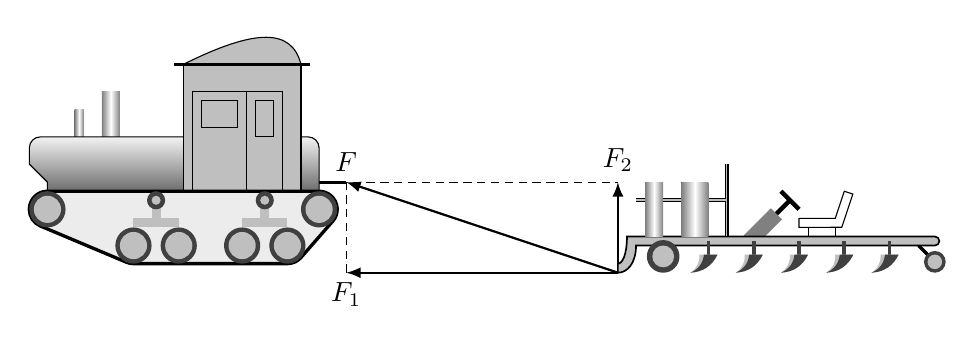
\begin{tikzpicture}[>=latex,scale=1.15]
  % \useasboundingbox(-1,-0.75)rectangle(3.7,1.4);
  \draw[->,thick](0,0)--(0,1)node[above]{$F_2$};
  \draw[->,thick](0,0)--(-3,0)node[below]{$F_1$};
  \draw[->,thick](0,0)--(-3,1)node[above]{$F$};
  \draw[thin,densely dashed](-3,0)--(-3,1)--(0,1);
  \draw[very thick](3.32,0.3)--(3.5,0.12);
  \draw[ultra thick](1.5,0.4)--++(0.4,0.4)(1.8,0.9)--(2.0,0.7);
  \draw[line width=2mm ,gray](1.45,0.35)--++(0.3,0.3);
  \draw(2,0.5)--++(0,0.1)--++(0.4,0)--++(0.1,0.3)--++(0.0949,-0.0316)--++(-0.1228,-0.3664)--cycle;
  \draw(2.1,0.5)rectangle(2.4,0.4);
  \draw[semithick,fill=lightgray](0,0)--(0,0.1)..controls(0.05,0.1)and(0.1,0.2)..(0.1,0.4)--(3.5,0.4)arc(90:-90:0.05)--(0.2,0.3)..controls(0.2,0.1)and(0.1,0)..cycle;
  \fill[darkgray](0.5,0.18)circle(0.18);
  \fill[lightgray](0.5,0.18)circle(0.12);
  \foreach \x in {1,1.5,...,3}
  {
    \fill[darkgray](\x-0.02,0.35)rectangle(\x+0.02,0.2);
    \fill[lightgray](\x-0.2,0)to[bend right](\x-0.1,0.2)--(\x+0.1,0.2)to[bend left]cycle;
    \fill[darkgray](\x-0.2,0)to[bend right](\x-0.05,0.2)--(\x+0.1,0.2)to[bend left]cycle;
  }
  \fill[darkgray](3.5,0.12)circle(0.12);
  \fill[lightgray](3.5,0.12)circle(0.08);
  \draw[double=lightgray](0.2,0.8)--++(1,0)(1.2,0.4)--(1.2,1.2);
  \fill[left color=gray,right color=gray,middle color=white](0.3,0.4)rectangle(0.5,1.0);
  \fill[left color=gray,right color=gray,middle color=white](0.7,0.4)rectangle(1.0,1.0);
  \fill[left color=gray,right color=gray,middle color=white](-6,1.2)rectangle(-5.9,1.8);
  \fill[left color=gray,right color=gray,middle color=white](-5.7,1.2)rectangle(-5.5,2.0);
  \draw[top color=lightgray!20,bottom color= darkgray](-6.3,0.7)--++(0,0.3)--++(-0.2,0.2)[rounded corners]--++(0,0.3)--++(3.2,0)--++(0,-0.8)--cycle;
  \draw[fill=lightgray](-4.8,0.7)rectangle(-3.5,2.3);
  \draw(-4.7,0.7)rectangle(-3.7,2.0)(-4.1,0.7)--(-4.1,2.0);
  \draw(-4.6,1.6)rectangle(-4.2,1.9)(-4.0,1.5)rectangle(-3.8,1.9);

  \draw[fill=lightgray](-4.8,2.3)..controls (-4.0,2.7) and (-3.6,2.7)..(-3.5,2.3);
  \draw[very thick](-4.9,2.3)--(-3.4,2.3)(-3,1)--(-3.3,1);
  \draw[fill=lightgray!30,very thick](-5.35,0.1)--(-3.65,0.1)arc(-90:-41.186:0.2)--++(0.35,0.4)arc(-41.186:90:0.2)--(-6.3,0.9)arc(90:247.166:0.2)--++(0.95,-0.4)arc(247.166:270:0.2);
  \fill[darkgray](-3.3,0.7)circle(0.2)(-6.3,0.7)circle(0.2);
  \fill[lightgray](-3.3,0.7)circle(0.15)(-6.3,0.7)circle(0.15);
  \foreach \x in {-5.1,-3.9}
  {
    \fill[darkgray](\x-0.25,0.3)circle(0.2)(\x+0.25,0.3)circle(0.2);
    \fill[lightgray](\x-0.25,0.3)circle(0.15)(\x+0.25,0.3)circle(0.15);
    \fill[lightgray](\x-0.25,0.5)rectangle(\x+0.25,0.6);
    \fill[lightgray](\x-0.05,0.5)rectangle(\x+0.05,0.8);
    \fill[darkgray](\x,0.8)circle(0.1);
    \fill[lightgray](\x,0.8)circle(0.05);
  }
  \end{tikzpicture}
\end{document}